% !TEX root = ./1-Sucesiones_Slides.tex

%! Datos del curso
\newcommand{\SIGLACURSO}{MAT013}
\newcommand{\NOMBRECURSO}{Matemática 3}
\newcommand{\PROFESOR}{Eduardo Hirsh}
\newcommand{\FECHA}{Primer Semestre 2026}
\newcommand{\FECHACORTO}{1er. Semestre 2026}

%! Datos presentación
\newcommand{\NOMBREDOCUMENTO}{Sucesiones y Series}
\author{\PROFESOR}
\title[\SIGLACURSO]{\SIGLACURSO\ - \NOMBRECURSO\\ \NOMBREDOCUMENTO}
\date[\FECHACORTO]{\FECHA}
\institute[]{}

\begin{document}

\only<article>{
%! Encabezado
\thispagestyle{empty}
\vspace*{-4cm}
\begin{center}
  
\includegraphics[scale=.75]{logo-dmat-vertical.pdf}
\end{center}
% \vspace{1mm}
% \noindent\rule[0mm]{175mm}{0.1mm}
%! Titulo
\begin{center}
  \textbf{\Large\SIGLACURSO\ - \NOMBRECURSO}\\[1mm]
  \textbf{\Large\NOMBREDOCUMENTO}\\
  {\large\PROFESOR}\\
  \FECHACORTO
\end{center}
\vspace{5mm}
}

\only<presentation>{
\begin{frame}
  \begin{center}
  
\includegraphics[scale=.6]{Logo_USM_MAT.pdf}
  \end{center}
  \titlepage
  % \begin{center}\includegraphics[scale=.20]{Logo_Depto.pdf}\end{center}
  \vspace{2cm}
\end{frame}
}

%! tabla de contenidos completa
\begin{frame}
\tableofcontents
\end{frame}

%! sección
\section{Sucesiones}
\begin{frame}
\sectionpage
\end{frame}

\begin{frame}
\tableofcontents[currentsection]
\end{frame}

%! subsección
\subsection{Definición y operatoria}
\begin{frame}
\subsectionpage
\end{frame}

% \begin{frame}
% \tableofcontents[currentsubsection]
% \end{frame}

\begin{frame}
  \begin{defn}
    Una \textbf{sucesión} es una función cuyo dominio es usualmente el conjunto de los números naturales $\Nat=\set{1,2,3,\ldots}$.
    $$\begin{array}{rcl}
      a:\Nat  & \longrightarrow & \Real \\
            n & \longmapsto     & a_n
    \end{array}$$
    Usualmente se denota por $\set{a_n}_{n\in\Nat}$, $\set{a_n}_{n=1}^{\infty}$ o simplemente $\set{a_n}$.
  \end{defn}
  \onslide<2->{
    \begin{rem}
      Se puede considerar sucesiones con dominio en $\Nat_0=\set{0,1,2,\ldots}$ o  incluso en $\Ent$, según convenga por motivos prácticos. por ejemplo,
      $$\begin{array}{rcl}
        a_{\cdot}:\Nat_0  & \longrightarrow & \Real \\
                        n & \longmapsto     & \dfrac{1}{2^n}
      \end{array}$$
      este caso lo podríamos denotar por $a=\set{\frac{1}{2^n}}_{n\in\Nat_0}=\set{\frac{1}{2^n}}_{n=0}^{\infty}$.
    \end{rem}
  }
\end{frame}

\begin{frame}
  Una sucesión se puede representar gráficamente como una secuencia de puntos en la recta real, por ejemplo la sucesión $\set{\frac{1}{n}}_{n=1}^{\infty}$ se puede representar como
  \vspace{-5mm}
  \begin{center}
    \hspace*{-10mm}\href{https://graficosucesiones1d.streamlit.app/}{
\includegraphics[scale=0.4]{./imagenes/Sucesion_1D.png}}
  \end{center}
  \onslide<2->{
    \vspace{-2mm}
    También se puede representar como una secuencia de puntos en el plano como
    \vspace{-5mm}
    \begin{center}
      \href{https://graficosucesiones2d.streamlit.app/}{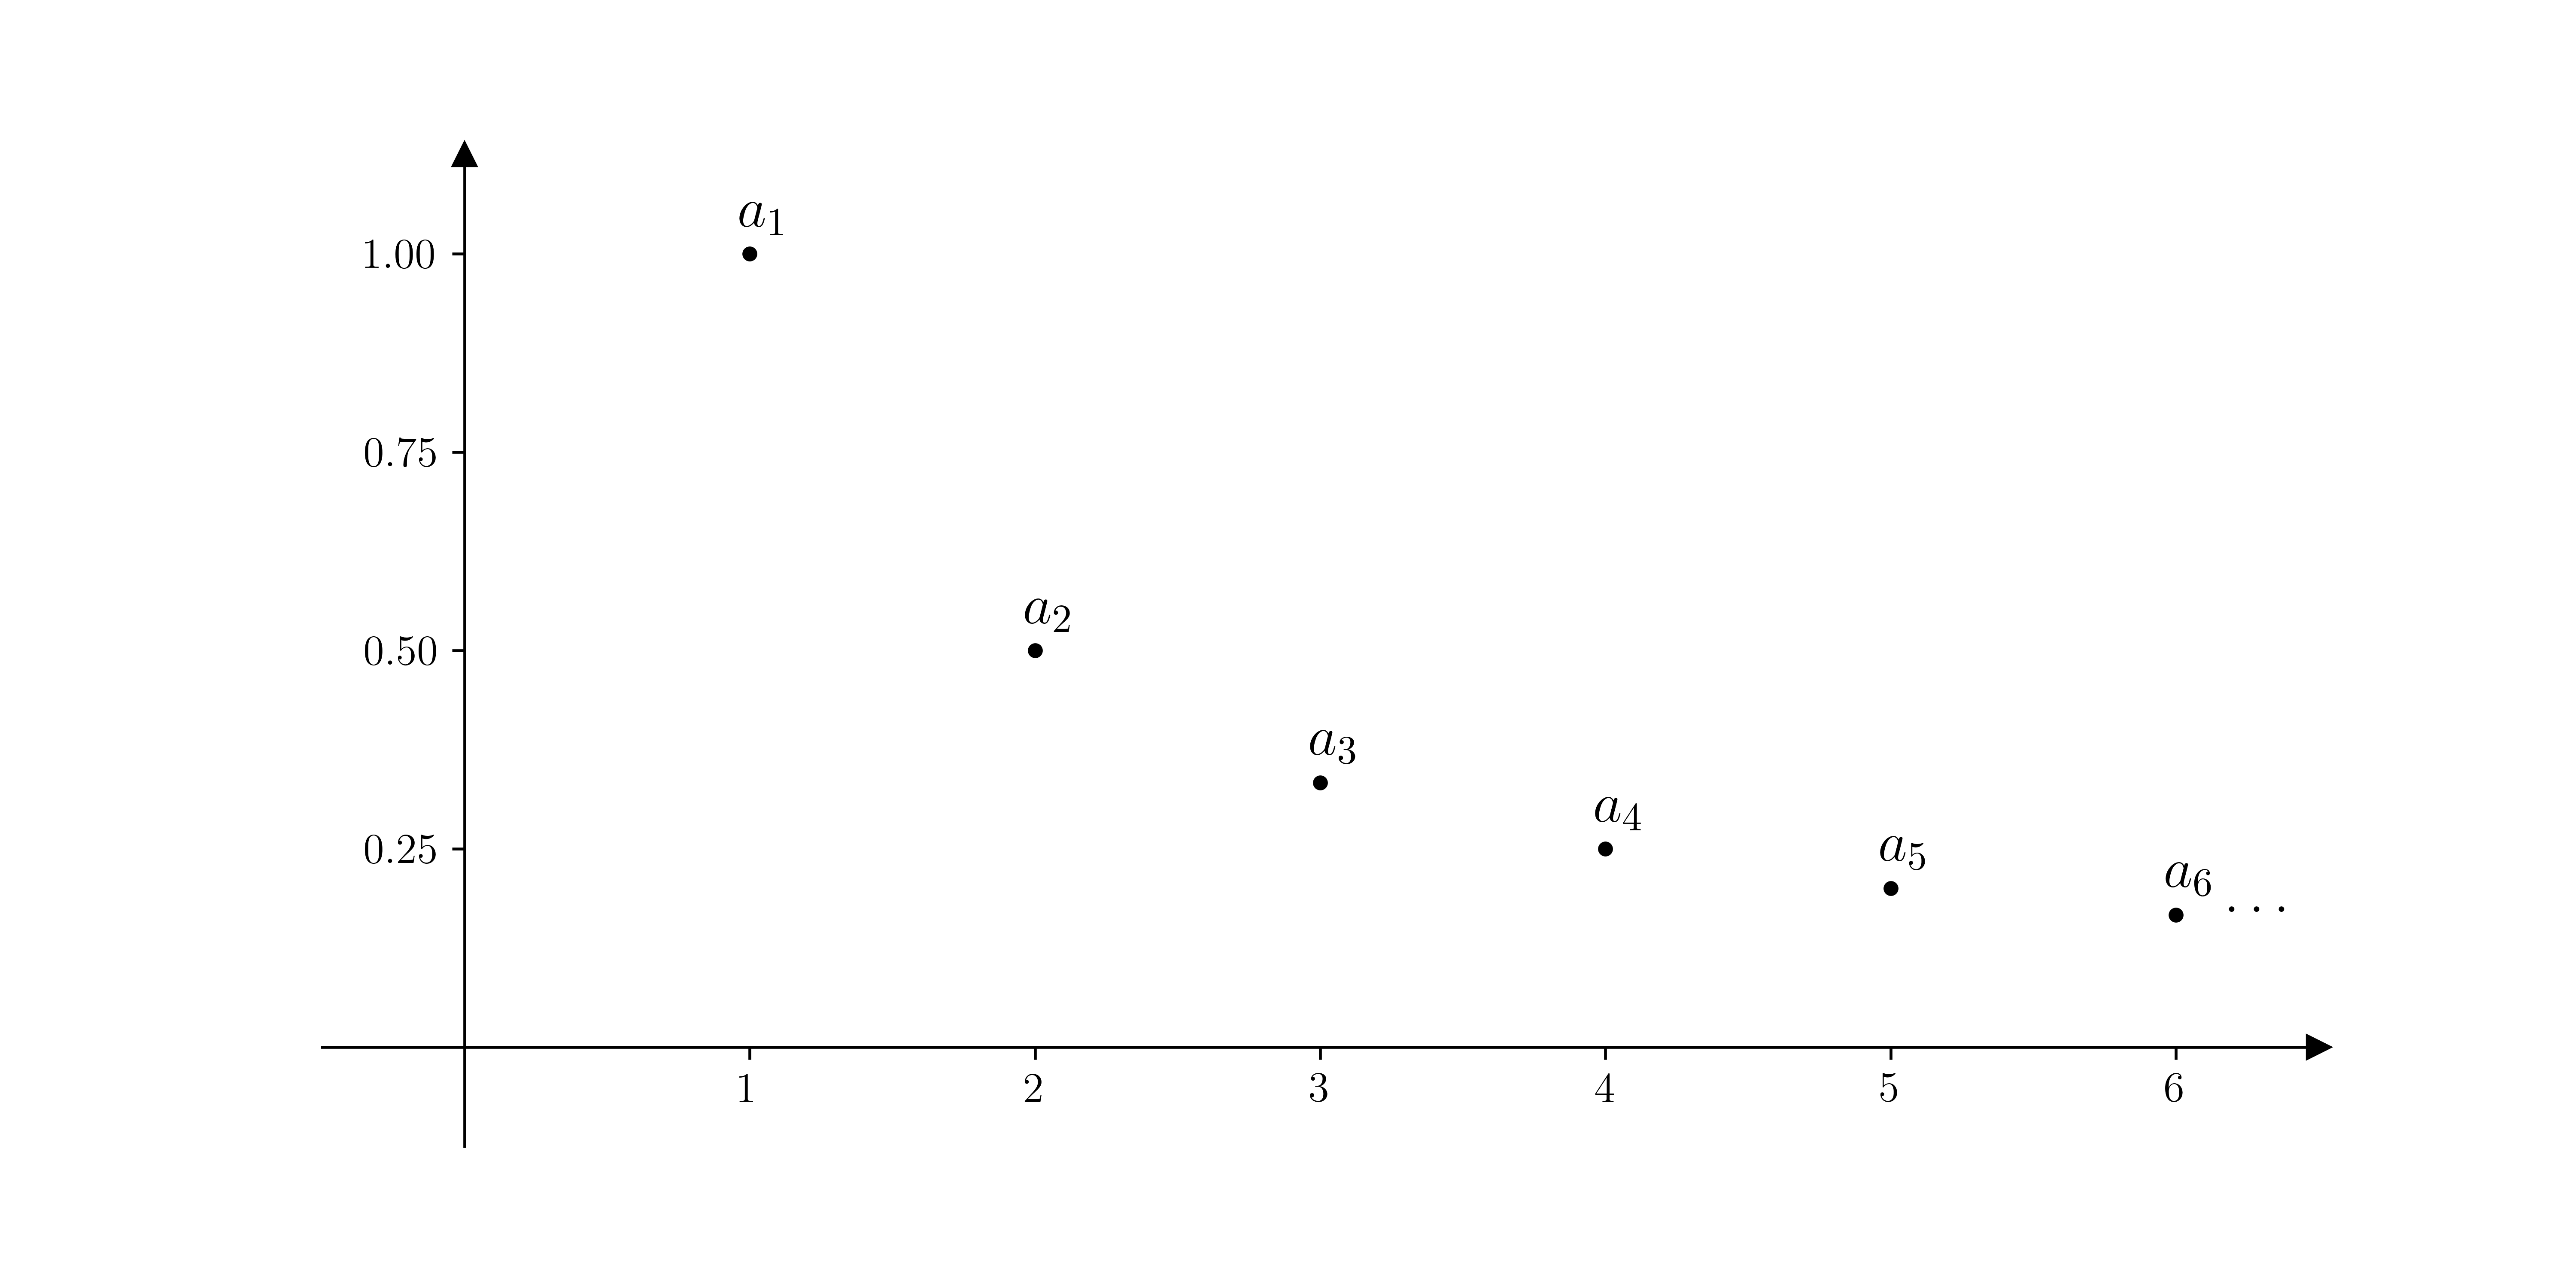
\includegraphics[scale=0.4]{./imagenes/Sucesion_2D.png}}
    \end{center}
  }
\end{frame}

\begin{frame}
  \begin{egs}
    Algunos ejemplos de sucesiones son:\\[0.5cm]
    \begin{enumerate}[<+->]
      \item La sucesión constante $a_n=c$.\\[0.25cm]
      \item La sucesión aritmética $a_n=a_0+nd$.\\[0.25cm]
      \item La sucesión geométrica $a_n=a_0\cdot r^n$.\\[0.25cm]
      \item La sucesión armónica $a_n=\dfrac{1}{n}$.\\[0.25cm]
      \item La sucesión de Fibonacci $a_n=a_{n-1}+a_{n-2}$ y $a_0=a_1=1$.\\[0.25cm]
    \end{enumerate}
  \end{egs}
\end{frame}

\begin{frame}
  Existen varios métodos para definir los términos de una sucesión, los principales son:\\[0.5cm]
  \begin{enumerate}
    \item<2-> Definición directa: Se da una fórmula que permite calcular el término $n$-ésimo de la sucesión.\\[0.25cm]
    \item<3-> Definición recursiva: Se dan términos iniciales y una regla que permite calcular el término $n$-ésimo en función de los términos anteriores.\\[0.25cm]
  \end{enumerate}
  \onslide<4->{
    \begin{eg}
      La sucesión aritmética se puede definir de forma directa como $a_n=a_0+nd$ o de forma recursiva como $a_0=a_0$ y $a_{n+1}=a_n+d$.
    \end{eg}
  }
\end{frame}

\begin{frame}
  Se pueden definir operaciones entre sucesiones, las principales son:\\[0.5cm]
  \begin{enumerate}
    \item<2-> Suma de sucesiones: $\set{a_n}+\set{b_n}=\set{a_n+b_n}$.\\[0.25cm]
    \item<3-> Resta de sucesiones: $\set{a_n}-\set{b_n}=\set{a_n-b_n}$.\\[0.25cm]
    \item<4-> Multiplicación escalar: $c\cdot\set{a_n}=\set{c\cdot a_n}$.\\[0.25cm]
    \item<5-> Multiplicación de sucesiones: $\set{a_n}\cdot\set{b_n}=\set{a_n\cdot b_n}$.\\[0.25cm]
    \item<6-> División de sucesiones: $\dfrac{\set{a_n}}{\set{b_n}}=\set{\dfrac{a_n}{b_n}}$.\\[0.25cm]
  \end{enumerate}
\end{frame}


%! subsección
\subsection{Límites de Sucesiones}
\begin{frame}
\subsectionpage
\end{frame}

% \begin{frame}
% \tableofcontents[currentsubsection]
% \end{frame}

\begin{frame}
  \begin{defn}
    Sea $\set{a_n}$ una sucesión, se dice que $\set{a_n}$ \textbf{converge} a un número $L\in\Real$ si se cumple
    $$\forall\varepsilon>0\quad\exists N\in\Nat\quad\forall n\in\Nat\quad n\geq N\Rightarrow\abs{a_n-L}<\varepsilon.$$
    En este caso se denota por
    $$\lim_{n\to\infty}a_n=L\quad\text{o}\quad a_n\to L\quad\text{cuando}\quad n\to\infty.$$
  \end{defn}
  \onslide<2->{
    \begin{rem}
      Si una sucesión no converge, se dice que \textbf{diverge}.
    \end{rem}
  }
\end{frame}

\begin{frame}
  \begin{defn}
    Sea $\set{a_n}$ una sucesión, se dice que $\set{a_n}$ \textbf{diverge a infinito} si se cumple
    $$\forall M>0\quad\exists N\in\Nat\quad\forall n\in\Nat\quad n\geq N\Rightarrow a_n>M.$$
    En este caso se denota por
    $$\lim_{n\to\infty}a_n=\infty\quad\text{o}\quad a_n\to\infty\quad\text{cuando}\quad n\to\infty.$$
  \end{defn}
  \onslide<2->{
    \begin{defn}
      Sea $\set{a_n}$ una sucesión, se dice que $\set{a_n}$ \textbf{diverge a menos infinito} si se cumple
      $$\forall M>0\quad\exists N\in\Nat\quad\forall n\in\Nat\quad n\geq N\Rightarrow a_n<-M.$$
      En este caso se denota por
      $$\lim_{n\to\infty}a_n=-\infty\quad\text{o}\quad a_n\to-\infty\quad\text{cuando}\quad n\to\infty.$$
    \end{defn}
  }
\end{frame}

\begin{frame}
  \begin{prop}
    Sean $\set{a_n}$ y $\set{b_n}$ sucesiones que convergen a $L$ y $M$ respectivamente, y $c\in\Real$ una constante, entonces se cumplen las siguientes propiedades:\\[0.5cm]
    \begin{enumerate}
      \item<2-> $\lim\limits_{n\to\infty}(a_n+b_n)=L+M$.\\[0.25cm]
      \item<3-> $\lim\limits_{n\to\infty}(a_n-b_n)=L-M$.\\[0.25cm]
      \item<4-> $\lim\limits_{n\to\infty}c\cdot a_n=c\cdot L$.\\[0.25cm]
      \item<5-> $\lim\limits_{n\to\infty}(a_n\cdot b_n)=L\cdot M$.\\[0.25cm]
      \item<6-> $\lim\limits_{n\to\infty}\dfrac{a_n}{b_n}=\dfrac{L}{M}$, si $M\neq 0$.\\[0.25cm]
    \end{enumerate}
  \end{prop}
\end{frame}

\begin{frame}
  \begin{thm}
    Si $a_n\leq b_n\leq c_n$ y $\lim_{n\to\infty}a_n=\lim_{n\to\infty}c_n=L$, entonces $\lim_{n\to\infty}b_n=L$
  \end{thm}
  \onslide<2->{
    \begin{center}
      \href{https://sucesionesteoremasandwich.streamlit.app/}{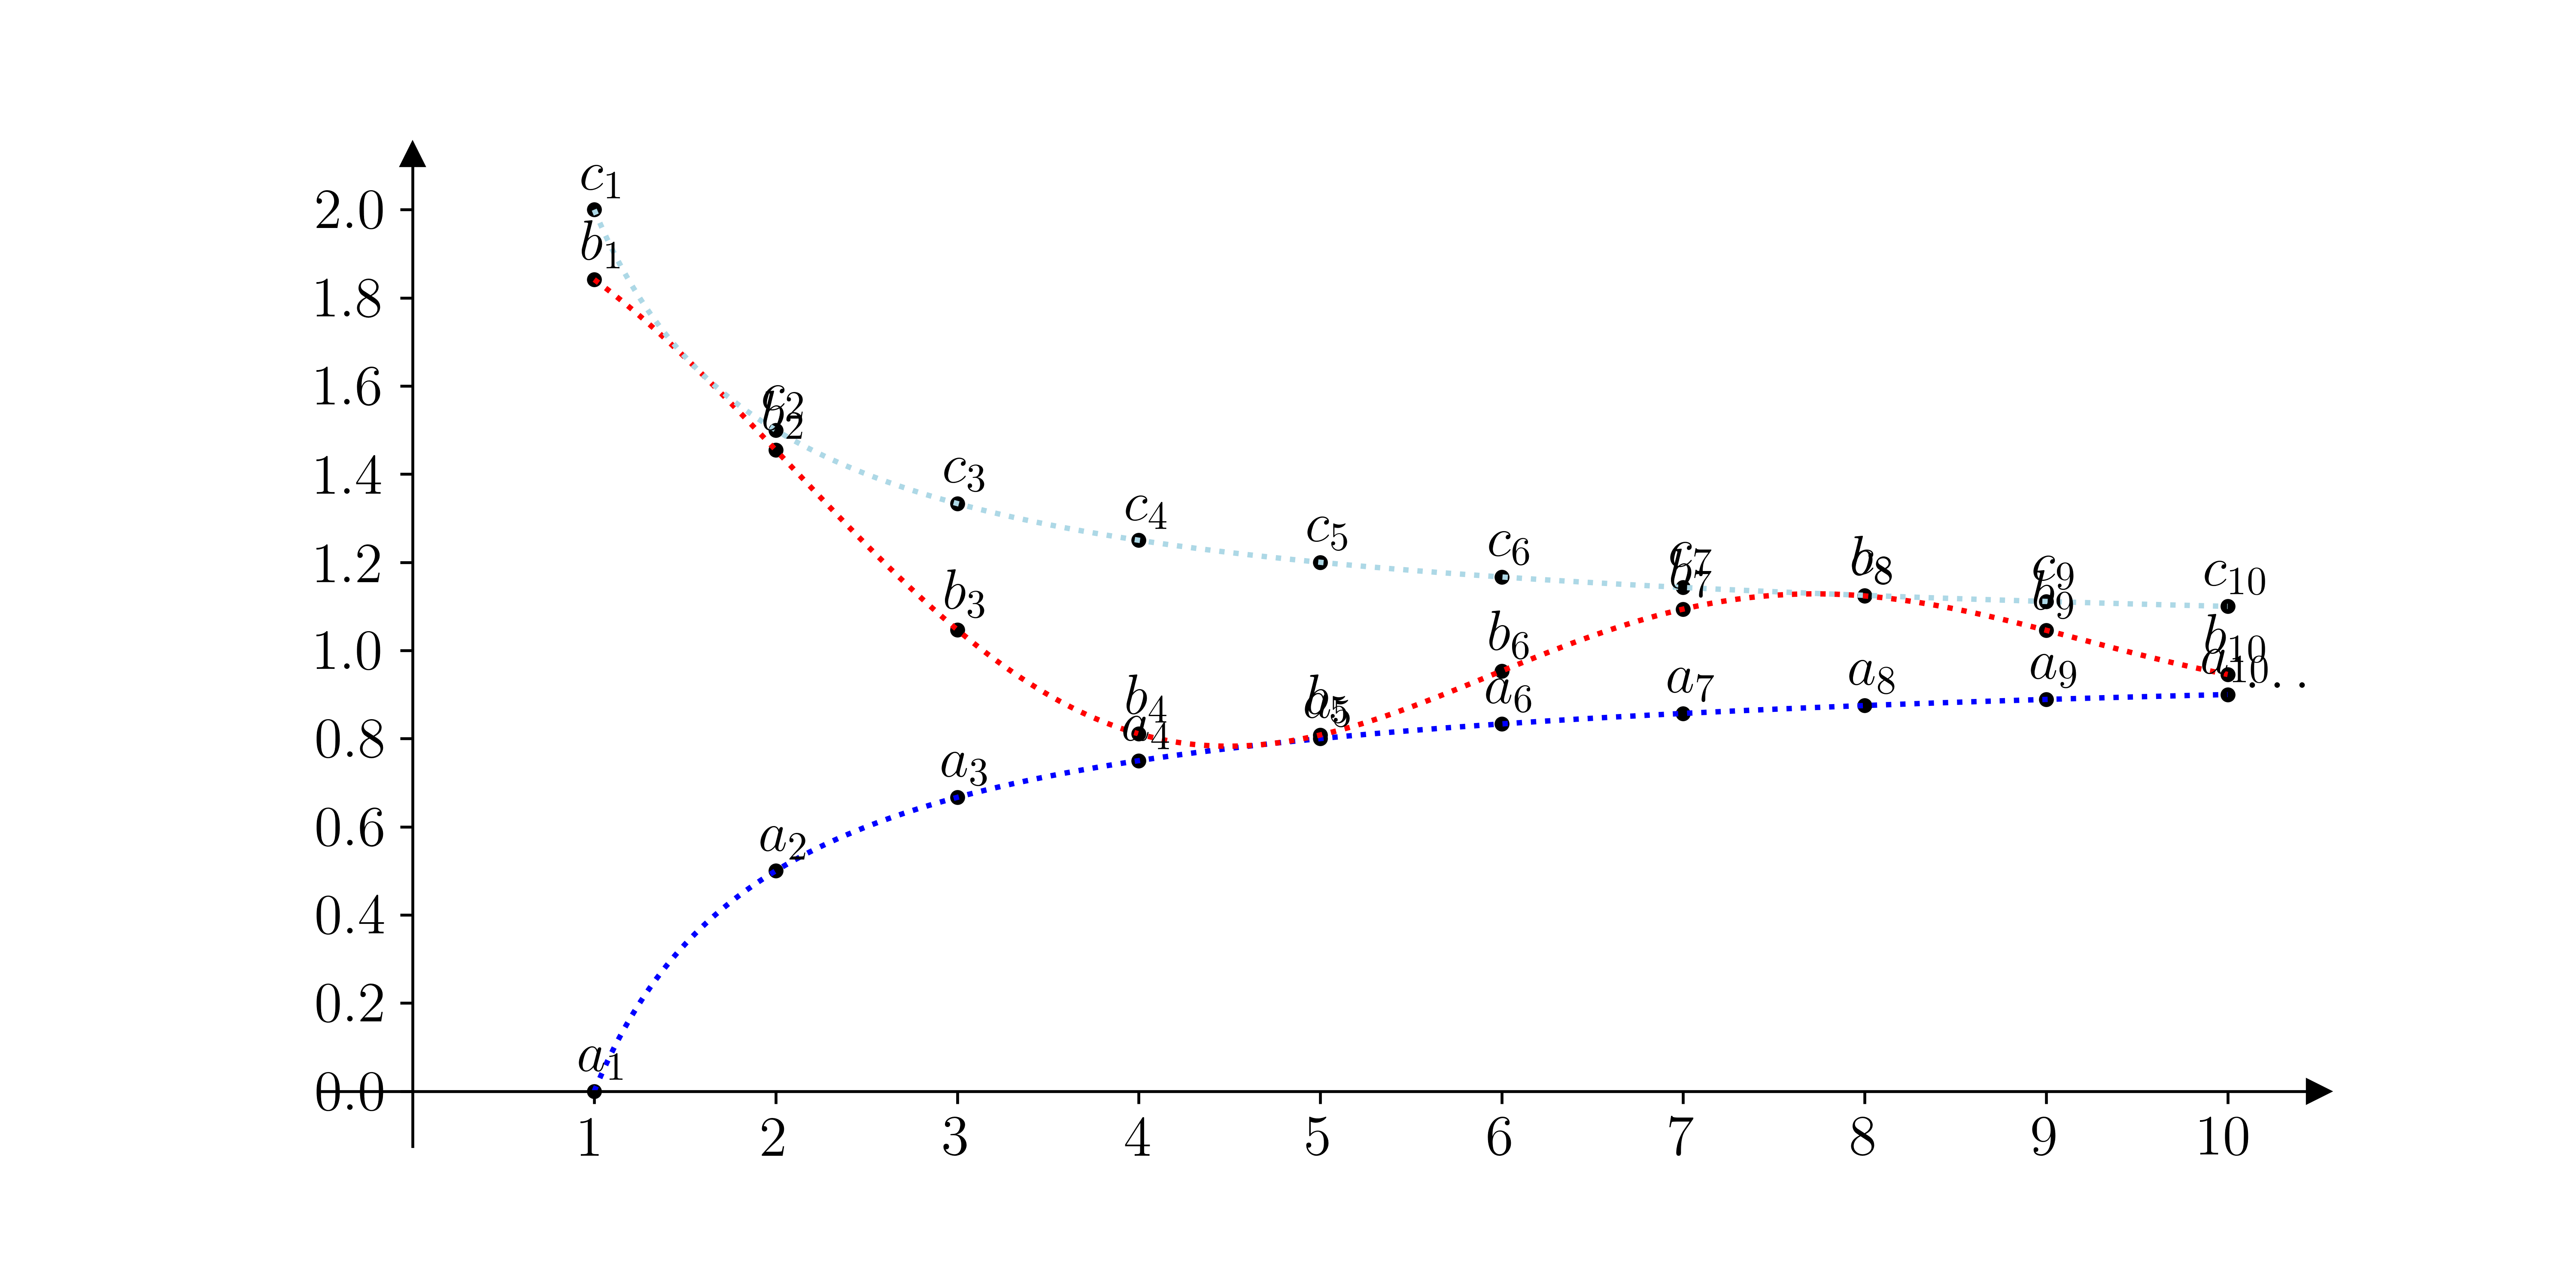
\includegraphics[scale=0.4]{./imagenes/Teorema_Sandwich.png}}
    \end{center}
  }
\end{frame}

\begin{frame}
  \begin{thm}
    Son equivalentes las siguientes afirmaciones:
    \begin{enumerate}
      \item $\lim\limits_{n\to\infty}a_n=L$.
      \item $\lim\limits_{n\to\infty}\abs{a_n-L}=0$.
      \item $\lim\limits_{n\to\infty}(a_n-L)=0$.
    \end{enumerate}
  \end{thm}
  \onslide<2->{
    \begin{thm}
      Si $\lim\limits_{n\to\infty}a_n=L$ y $f:\Real\to\Real$ es una función continua en $L$, entonces 
      $$\lim\limits_{n\to\infty}f(a_n)=f(L)$$
    \end{thm}
    % \begin{thm}
    %   Toda sucesión monótona acotada es convergente.
    % \end{thm}
  }
\end{frame}

\begin{frame}
  \begin{thm}
    Sea $f:\Real\to\Real$ una función real tal que $\lim\limits_{x\to\infty}f(x)=L$ y $\set{a_n}$ una sucesión definida por $a_n=f(n)$, entonces 
    $$\lim_{n\to\infty}a_n=L$$
  \end{thm}
  \onslide<2->{
    \begin{rem}
      Si $f$ diverge cuando $x\to\infty$, la sucesión dada por $a_n=f(n)$ podría converger.\\[0.25cm]
      Por ejemplo, si $f(x)=\cos(2x\pi)$, entonces
      $$\lim_{x\to\infty}f(x)\text{ no existe}$$
      pero
      $$\lim_{n\to\infty}f(n)=1$$ 
    \end{rem}
  }
\end{frame}

\begin{frame}
  \begin{defn}
    \begin{itemize}
      \item<1-> Una sucesión $\set{a_n}$ se dice que es \textbf{creciente} si $a_n\leq a_{n+1}$ para todo $n\in\Nat$.\\[0.25cm]
      \item<2-> Una sucesión $\set{a_n}$ se dice que es \textbf{decreciente} si $a_n\geq a_{n+1}$ para todo $n\in\Nat$.\\[0.25cm]
      \item<3-> Una sucesión $\set{a_n}$ se dice que es \textbf{monótona} si es creciente o decreciente.
    \end{itemize}
  \end{defn}
  \onslide<4->{
    \begin{thm}
      Toda sucesión creciente y acotada superiormente es convergente.
    \end{thm}
  }
  \onslide<5->{
    \begin{thm}
      Toda sucesión decreciente y acotada inferiormente es convergente.
    \end{thm}
  }
  \onslide<6->{
    \begin{thm}
      Toda sucesión monótona y acotada es convergente.
    \end{thm}
  }
\end{frame}

\begin{frame}
  \begin{eg}
    La sucesión dada por $a_n=1-\frac{1}{n}$ es creciente y acotada superiormente por $1$, entonces $\set{a_n}$ es convergente. Gráficamente.
    \vspace{-3mm}
    \begin{center}
      \href{https://sucesionesmonotonaacotada.streamlit.app/}{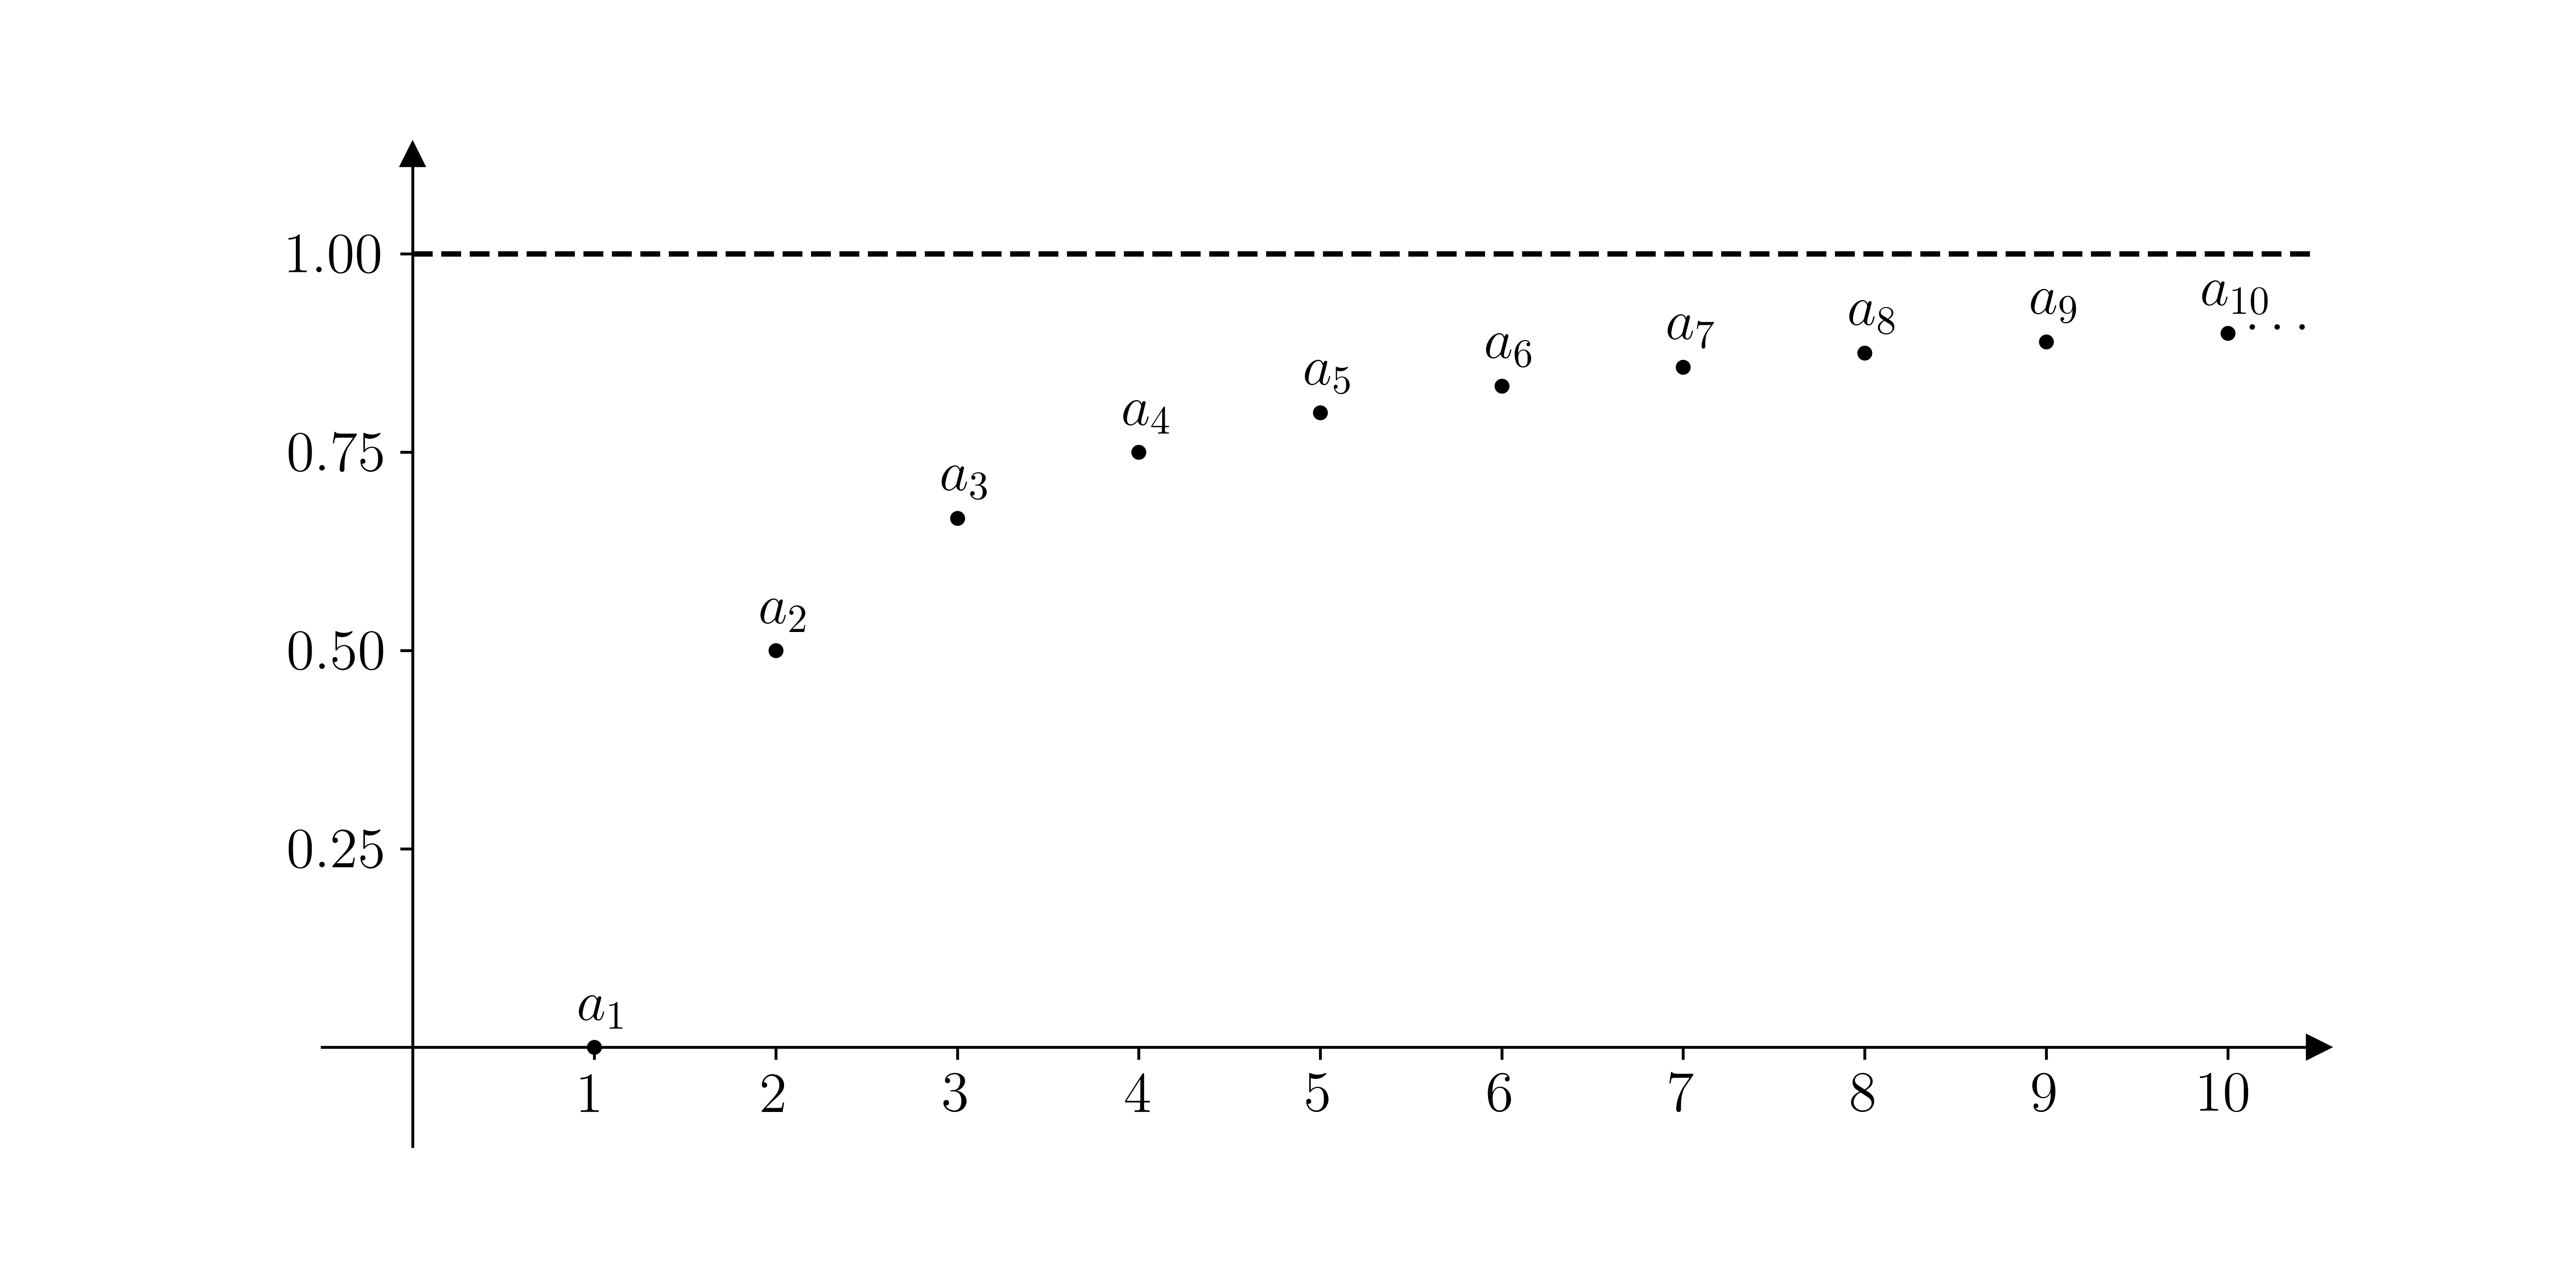
\includegraphics[scale=0.4]{./imagenes/Sucesion_Creciente_Acotada.png}}
    \end{center}
  \end{eg}
\end{frame}

\begin{frame}
  \begin{egs}
    \vspace{2mm}
    Calcule los siguientes límites.\\[0.25cm]
    \begin{enumerate}[<+->]
      \item $\displaystyle\lim_{n\to\infty}\dfrac{2n+5}{3n+1}$\\[3mm]
      \item $\displaystyle\lim_{n\to\infty}\dfrac{3n+2}{n^2+1}$\\[3mm]
      \item $\displaystyle\lim_{n\to\infty}\frac{\sqrt{n^2+n}}{n+1}$
    \end{enumerate}
  \end{egs}
\end{frame}

%! subsección
\subsection{Ejercicios}
\begin{frame}
\subsectionpage
\end{frame}

% \begin{frame}
% \tableofcontents[currentsubsection]
% \end{frame}

\begin{frame}
  Calcule los siguientes límites.\\[0.25cm]
  \begin{enumerate}
    \item $\displaystyle\lim_{n\to\infty}\dfrac{n^2+2n+5}{n^2+1}$\\
    \item $\displaystyle\lim_{n\to\infty}\dfrac{-2n+1}{n^2+n}$\\
    \item $\displaystyle\lim_{n\to\infty}\dfrac{n^2+2n-1}{n+1}$\\
    \item $\displaystyle\lim_{n\to\infty}\dfrac{3n^2+2n+1}{n^3-1}$\\
    \item $\displaystyle\lim_{n\to\infty}\dfrac{\sqrt{n}}{1+\sqrt{n}}$\\
    \item $\displaystyle\lim_{n\to\infty}\cos\left(\dfrac{2}{n}\right)$\\
    \item $\displaystyle\lim_{n\to\infty}\ln(n+1)-\ln(n)$\\
    \item $\displaystyle\lim_{n\to\infty}\sqrt{n}-\sqrt{n^2-1}$
  \end{enumerate}
\end{frame}

%! sección
\section{Series}
\begin{frame}
\sectionpage
\end{frame}

\begin{frame}
\tableofcontents[currentsection]
\end{frame}

%! subsección
\subsection{Definición}
\begin{frame}
\subsectionpage
\end{frame}

% \begin{frame}
% \tableofcontents[currentsubsection]
% \end{frame}

\begin{frame}
  El concepto de serie busca construir una definición de suma infinita, informalmente
  $$a_1+a_2+a_3+\cdots+a_n+\cdots$$
  para esto haremos algunas definiciones que nos permitan formalizar este concepto. Usaremos la notación de sumatoria para representar la serie, incluso si esta suma no hace sentido. Que se denotará por
  $$\sum_{n=1}^{\infty}a_n=a_1+a_2+a_3+\cdots+a_n+\cdots$$
\end{frame}

\begin{frame}
  \begin{defn}
    Dada una sucesión $\set{a_n}$, se define las \textbf{sumas parciales} de la serie como
    $$S_n=\sum_{k=1}^{n}a_k=a_1+a_2+\cdots+a_n$$
  \end{defn}
  \onslide<2->{
    \begin{defn}
      Diremos que una serie \textbf{converge} a un número $S$ si la sucesión de sumas parciales $\set{S_n}$ converge a $S$, es decir
      $$\lim_{n\to\infty}S_n=S$$
      En cuyo caso se denotará por
      $$\sum_{n=1}^{\infty}a_n=S$$
      En caso contrario diremos que la serie \textbf{diverge}.
    \end{defn}
  }
\end{frame}

\begin{frame}
  \begin{egs}
    \vspace{3mm}
    \begin{itemize}[<+->]
      \item $\displaystyle\sum_{n=1}^{\infty}\frac{1}{2^n}=1$\\[0.5cm]
      \item $\displaystyle\sum_{n=1}^{\infty}(-1)^n$ diverge\\[0.5cm]
      \item $\displaystyle\sum_{n=1}^{\infty}\frac{1}{n}$ diverge\\[0.5cm]
    \end{itemize}
  \end{egs}
\end{frame}

\begin{frame}
  La serie geométrica es
  $$\sum_{n=0}^{\infty}r^n=1+r+r^2+\ldots$$
  \onslide<2->{
    Si $\abs{r}<1$ entonces la serie converge a
    $$\sum_{n=0}^{\infty}r^n=\dfrac{1}{1-r}$$
  }
  \onslide<3->{
    Si $\abs{r}\geq 1$ entonces la serie diverge, si además $r> 1$ entonces la serie diverge a infinito. y lo denotaremos por
    $$\sum_{n=0}^{\infty}r^n=\infty$$
  }
\end{frame}

\begin{frame}
  \begin{prop}
    Sean $\sum_{n=1}^{\infty}a_n$ y $\sum_{n=1}^{\infty}b_n$ series convergentes, y $c\in\Real$ una constante, entonces se cumplen las siguientes propiedades:\\[0.5cm]
    \begin{enumerate}
      \item<2-> $\sum_{n=1}^{\infty}(a_n+b_n)=\sum_{n=1}^{\infty}a_n+\sum_{n=1}^{\infty}b_n$.\\[0.25cm]
      \item<3-> $\sum_{n=1}^{\infty}c\cdot a_n=c\cdot\sum_{n=1}^{\infty}a_n$.\\[0.25cm]
      \item<4-> $\sum_{n=1}^{\infty}(a_n-b_n)=\sum_{n=1}^{\infty}a_n-\sum_{n=1}^{\infty}b_n$.\\[0.25cm]
      % \item<5-> $\sum_{n=1}^{\infty}a_n\cdot b_n=\left(\sum_{n=1}^{\infty}a_n\right)\cdot\left(\sum_{n=1}^{\infty}b_n\right)$.\\[0.25cm]
      % \item<6-> $\sum_{n=1}^{\infty}a_n\cdot c=\left(\sum_{n=1}^{\infty}a_n\right)\cdot c$.\\[0.25cm]
      % \item<7-> $\sum_{n=1}^{\infty}c=\infty$ si $c\neq 0$.
    \end{enumerate}
  \end{prop}
\end{frame}

\begin{frame}
  \begin{thm}
    Si $\sum_{n=1}^{\infty}a_n$ converge, entonces $\lim_{n\to\infty}a_n=0$.
  \end{thm}
  \onslide<2->{
    \begin{cor}
      Si $\lim_{n\to\infty}a_n$ no existe o es distinto de cero, entonces $\sum_{n=1}^{\infty}a_n$ diverge.
    \end{cor}
  }
\end{frame}

\begin{frame}
  \begin{egs}
    Determine si las siguientes series convergen y en el caso que converjan calcule.
    \begin{itemize}[<+->]
      \item $\displaystyle\sum_{n=1}^{\infty}\dfrac{e^n}{3^{n-1}}$
      \item $\displaystyle\sum_{n=1}^{\infty}\dfrac{(n+1)^2}{n(n+2)}$
      %\item $\displaystyle\sum_{n=1}^{\infty}\ln\left(\frac{n}{2n+5}\right)$
      %\item $\displaystyle\sum_{n=1}^{\infty}(cos(1))^n$
      \item $\displaystyle\sum_{n=1}^{\infty}\frac{1}{n(n+1)}+\frac{12}{5^n}$\\
      \item $\displaystyle\sum_{n=1}^{\infty}\frac{1}{2^n}+\frac{1}{n}$\\
    \end{itemize}
  \end{egs}
\end{frame}

%! subsección
\subsection{Criterios de Convergencia}
\begin{frame}
\subsectionpage
\end{frame}

% \begin{frame}
% \tableofcontents[currentsubsection]
% \end{frame}

\begin{frame}
  \begin{thm}[Criterio de la Integral]
    Sea $f:\intervaloCA{1,\infty}\to\Real$ una función continua, no negativa y decreciente, $\set{a_n}$ una sucesión tal que $a_n=f(n)$, entonces la serie $\sum_{n=1}^{\infty}a_n$ converge si y solo si la integral
    $$\int_{1}^{\infty}f(x)dx$$
    converge.
  \end{thm}
  \onslide<2->{
    \vspace{-0.7cm}
    \begin{center}
      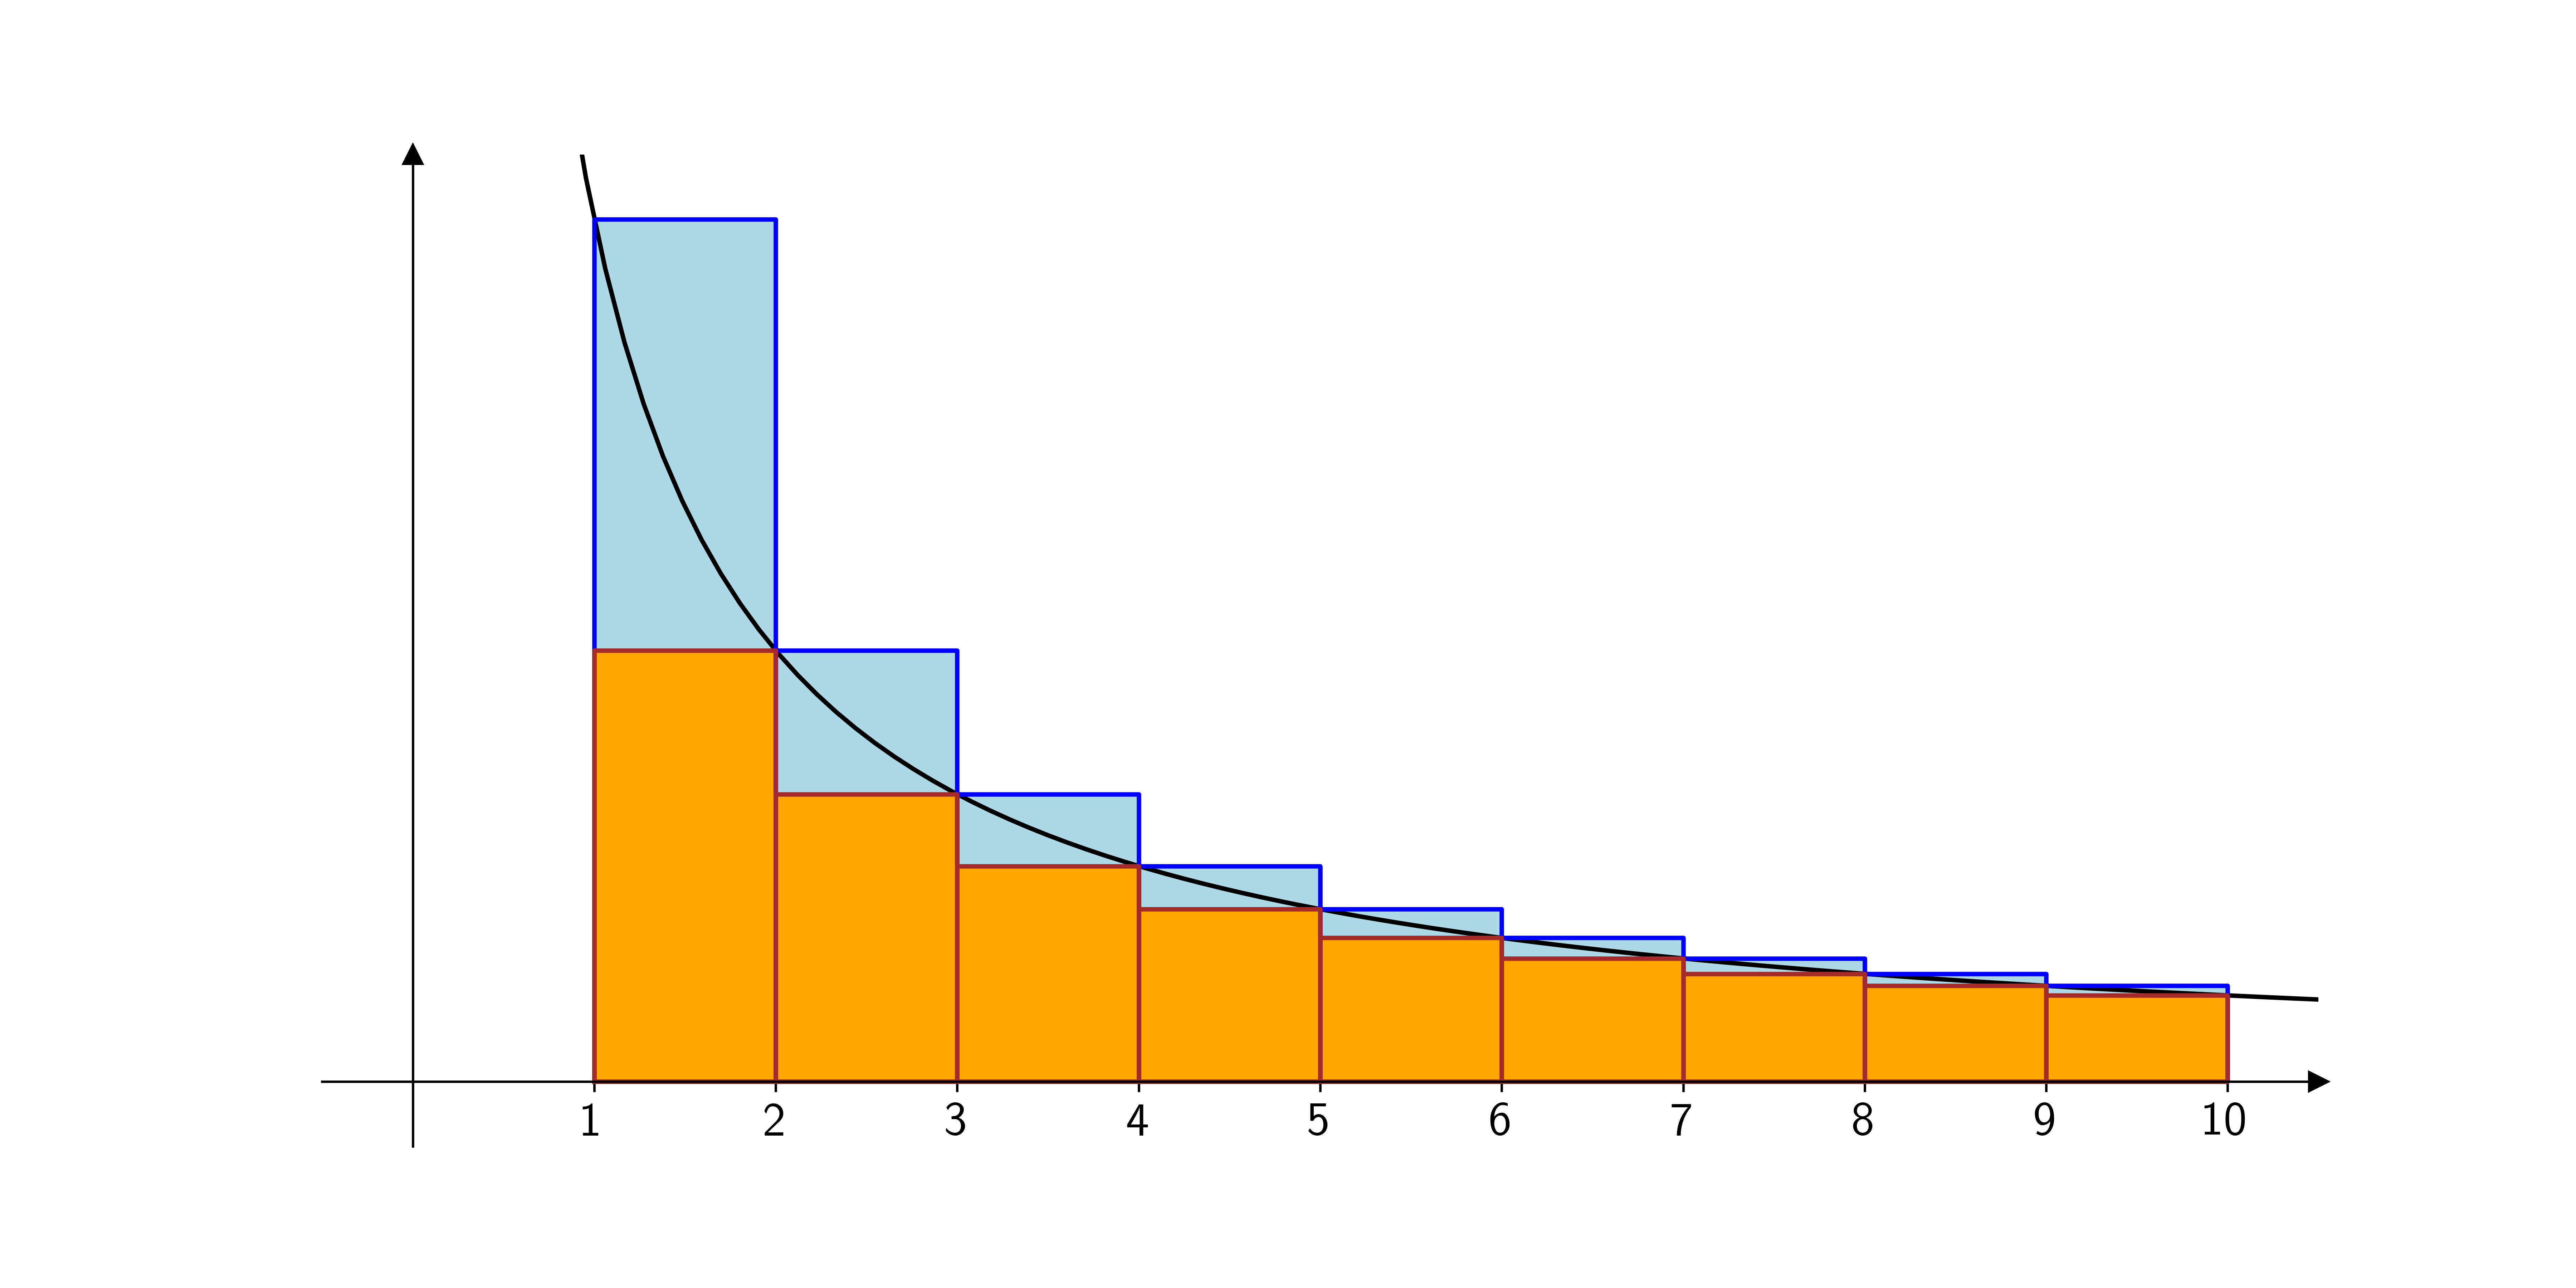
\includegraphics[scale=0.33]{./imagenes/CriterioIntegral_Sup_Inf.png}
    \end{center}
  }
\end{frame}

\begin{frame}
  \begin{egs}
    \begin{itemize}[<+->]
      \item ¿Para que valores de $p$ la serie $\displaystyle\sum_{n=1}^{\infty}\dfrac{1}{n^p}$ converge?\\[0.5cm]
      \item Determine si las siguientes series convergen o divergen.\\[0.5cm]
      \begin{enumerate}
        \item $\displaystyle\sum_{n=2}^{\infty}\dfrac{1}{n\ln(n)}$\\[0.25cm]
        \item $\displaystyle\sum_{n=1}^{\infty}\dfrac{\ln{n}}{n^2}$\\[0.25cm]
      \end{enumerate}
    \end{itemize}
  \end{egs}
\end{frame}

\begin{frame}
  \begin{thm}[Criterio de Comparación Ordinaria]
    Sean $\set{a_n}$ y $\set{b_n}$ dos sucesiones tales que $0\leq a_n\leq b_n$ para todo $n\in\Nat$, entonces\\[0.5cm]
    \begin{enumerate}
      \item Si $\sum_{n=1}^{\infty}b_n$ converge, entonces $\sum_{n=1}^{\infty}a_n$ converge.\\[0.25cm]
      \item Si $\sum_{n=1}^{\infty}a_n$ diverge, entonces $\sum_{n=1}^{\infty}b_n$ diverge.
    \end{enumerate}
  \end{thm}
\end{frame}

\begin{frame}
  \begin{egs}
    \begin{itemize}[<+->]
      \item la serie $\displaystyle\sum\frac{1}{n^2+1}$ converge.
      \vspace{0.5cm}
      \item la serie $\displaystyle\sum\frac{n+1}{n^2}$ diverge.
    \end{itemize}
  \end{egs}
\end{frame}

\begin{frame}
  \begin{thm}[Criterio de Comparación al Límite]
    Sean $\set{a_n}$ y $\set{b_n}$ dos sucesiones tales que $a_n,b_n>0$ para todo $n\in\Nat$, entonces\\[0.5cm]
    \begin{enumerate}
      \item Si $\lim_{n\to\infty}\dfrac{a_n}{b_n}=L\in\Real^+$, entonces $\sum_{n=1}^{\infty}a_n$ y $\sum_{n=1}^{\infty}b_n$ convergen o divergen simultáneamente.\\[0.25cm]
      \item Si $\lim_{n\to\infty}\dfrac{a_n}{b_n}=0$ y $\sum_{n=1}^{\infty}b_n$ converge, entonces $\sum_{n=1}^{\infty}a_n$ converge.\\[0.25cm]
      \item Si $\lim_{n\to\infty}\dfrac{a_n}{b_n}=\infty$ y $\sum_{n=1}^{\infty}b_n$ diverge, entonces $\sum_{n=1}^{\infty}a_n$ diverge.
    \end{enumerate}    
  \end{thm}
\end{frame}

\begin{frame}{Ejempos}
  \begin{itemize}
    \item La serie $\displaystyle\sum\frac{n+2}{n^2-n-1}$ diverge
    \vspace{0.5cm}
    \item La serie $\displaystyle\sum\frac{n+1}{n^3+3n^2-n-1}$ converge
    \vspace{0.5cm}
    % \item La serie $\displaystyle\sum\frac{1}{\ln(n)}$ diverge.
  \end{itemize}
\end{frame}

\begin{frame}
  \begin{thm}[Criterio de la serie alternante]
    Dada una serie de la forma
    $$\sum_{n=1}^{\infty}(-1)^{n-1}b_n=b_1-b_2+b_3-b_4+\cdots$$
    con $b_n\geq 0$ para todo $n\in\Nat$. Si se cumplen las siguientes condiciones
    \begin{enumerate}
      \item $\lim_{n\to\infty}b_n=0$.
      \item $b_{n+1}\leq b_n$ para todo $n\in\Nat$.
    \end{enumerate}
    entonces la serie converge.
  \end{thm}
  \onslide<2->{
    \begin{eg}
      La serie armónica alternate $\displaystyle\sum_{n=1}^{\infty}\dfrac{(-1)^{n-1}}{n}$ es un ejemplo de serie alternante convergente.
    \end{eg}
  }
\end{frame}

\begin{frame}
  \begin{thm}[Error de la convergencia alternante]
    Sea $\sum_{n=1}^{\infty} (-1)^{n-1}b_n$, con $b_n>0$, una seria alternante si se satisfacen
    \begin{enumerate}
      \item $\lim_{n\to\infty}b_n=0$.
      \item $b_{n+1}\leq b_n$ para todo $n\in\Nat$.
    \end{enumerate}
    Entonces
    $$\abs{R_n}=\abs{s-s_n}\leq b_{n+1}$$
  \end{thm}
  \onslide<2->{
    \begin{eg}
      En la serie armónica alternante el error al aproximar la serie por $s_9$ esta dado por
        $$\abs{s-s_9}=\sum_{n=1}^{\infty} (-1)^{n-1}\dfrac{1}{n}-\sum_{n=1}^{9} (-1)^{n}\dfrac{1}{n}\leq\dfrac{1}{10}$$
    \end{eg}
  }
\end{frame}

\begin{frame}
  \begin{egs}
    Analice la convergencia de las series\\[0.5cm]
    \begin{enumerate}[<+->]
      \item $\displaystyle\sum_{n=1}^{\infty} (-1)^{n}\dfrac{2n}{4n^2+1}$\\[0.25cm]
      \item $\displaystyle\sum_{n=1}^{\infty} (-1)^{n}\dfrac{\ln(n)}{n}$\\[0.25cm]
      \item $\displaystyle\sum_{n=1}^{\infty} (-1)^{n}\sen\left(\dfrac{\pi}{n}\right)$\\[0.25cm]
      % \item $\displaystyle\sum_{n=1}^{\infty} (-1)^{n}\cos\left(\dfrac{\pi}{n}\right)$
      % \item $\displaystyle\sum_{n=1}^{\infty} \dfrac{\sen\left(n\frac{\pi}{2}\right)}{n!}$
    \end{enumerate}
  \end{egs}
\end{frame}

%! subsección
\subsection{Convergencia Absoluta y Condicional}
\begin{frame}
\subsectionpage
\end{frame}

% \begin{frame}
% \tableofcontents[currentsubsection]
% \end{frame}

\begin{frame}
  \begin{thm}
    Si $\sum\abs{a_n}$ converge, entonces $\sum a_n$ converge.
  \end{thm}
  \onslide<2->{
    \begin{defn}
      Diremos que una serie $\sum a_n$ es \emph{absolutamente convergente} si $\sum\abs{a_n}$ converge.
    \end{defn}
  }
  \onslide<3->{
    \begin{defn}
      Diremos que una serie $\sum a_n$ es \emph{convergente condicionalmente} si converge, pero no es absolutamente convergente.
    \end{defn}
  }
\end{frame}

\begin{frame}
  \begin{egs}
    \begin{itemize}[<+->]
      \item $\displaystyle\sum_{n=1}^{\infty}\dfrac{(-1)^{n-1}}{n}$ Converge condicionalmente\\
      \vspace{0.5cm}
      \item $\displaystyle\sum_{n=1}^{\infty}(-2)^{1-n}$ Converge absolutamente.\\
      \vspace{0.5cm}
      \item $\displaystyle\sum_{n=1}^{\infty}\dfrac{(-1)^{n-1}}{n^p}$ Converge absolutamente si $p>1$
    \end{itemize}
  \end{egs}
\end{frame}

\begin{frame}
  \begin{thm}[Criterio del Cuociente]
    \begin{itemize}
      \item Si $\lim_{n\to\infty}\abs{\dfrac{a_{n+1}}{a_n}}=L<1$, entonces la serie $\sum a_n$ es absolutamente convergente.\\
      \vspace{0.5cm}
      \item Si $\lim_{n\to\infty}\abs{\dfrac{a_{n+1}}{a_n}}=L>1$ o $\lim_{n\to\infty}\abs{\dfrac{a_{n+1}}{a_n}}=\infty$, entonces la serie $\sum a_n$ es divergente.\\
      \vspace{0.5cm}
      \item Si $\lim_{n\to\infty}\abs{\dfrac{a_{n+1}}{a_n}}=1$ el criterio no es concluyente.
    \end{itemize}
  \end{thm}
\end{frame}

\begin{frame}
  \begin{egs}
    Analice la convergencia de las siguientes series.
    \begin{itemize}[<+->]
      \item $\displaystyle \sum_{n=1}^{\infty}\dfrac{n^2}{(-5)^n}$\\
      \vspace{0.5cm}
      \item $\displaystyle \sum_{n=1}^{\infty}\dfrac{n^n}{n!}$\\
    \end{itemize}
  \end{egs}
\end{frame}

\begin{frame}
  \begin{thm}[Criterio de la Raíz]
    \begin{itemize}
      \item Si $\lim_{n\to\infty}\sqrt[n]{\abs{a_n}}=L<1$, entonces la serie $\sum a_n$ es absolutamente convergente.\\
      \vspace{0.5cm}
      \item Si $\lim_{n\to\infty}\sqrt[n]{\abs{a_n}}=L>1$ o $\lim_{n\to\infty}\sqrt[n]{\abs{a_n}}=\infty$, entonces la serie $\sum a_n$ es divergente.\\
      \vspace{0.5cm}
      \item Si $\lim_{n\to\infty}\sqrt[n]{\abs{a_n}}=1$ el criterio no es concluyente.
    \end{itemize}
  \end{thm}
\end{frame}

\begin{frame}
  \begin{egs}
    Analice la convergencia de las siguientes series.\\[0.5cm]
    \begin{itemize}[<+->]
      \item $\displaystyle \sum_{n=1}^{\infty}\left(\dfrac{3n+2}{7n+5}\right)^n$\\
      \vspace{0.25cm}
      \item $\displaystyle \sum_{n=1}^{\infty}\left(\dfrac{2n^3+2n-1}{n^3+2n^2-n}\right)^n$\\
    \end{itemize}
  \end{egs}
\end{frame}

\begin{frame}{Ejercicios}
  Estudie la convergencia de las siguientes series.\\[0.5cm]
  \begin{enumerate}
    \item $\displaystyle\sum_{n=1}^{\infty}\dfrac{(-2)^n}{n^4}$
    \vspace{0.25cm}
    \item $\displaystyle\sum_{n=1}^{\infty}e^{-n}n!$
    \vspace{0.25cm}
    \item $\displaystyle\sum_{n=1}^{\infty}\dfrac{n!}{n^n}$
    \vspace{0.25cm}
    \item $\displaystyle\sum_{n=1}^{\infty}\left(\dfrac{n^2+1}{2n^2+1}\right)^n$
  \end{enumerate}
\end{frame}

%! subsección
\subsection{Ejercicios}
\begin{frame}
\subsectionpage
\end{frame}

% \begin{frame}
% \tableofcontents[currentsubsection]
% \end{frame}

\begin{frame}
  \begin{enumerate}
    \item Determine usando la definición y propiedades básicas si las siguientes series convergen o divergen.
    \begin{multicols}{3}
      \begin{enumerate}
        \item $\displaystyle\sum_{n=1}^{\infty}\dfrac{2+5^n}{2^n}$
        \item $\displaystyle\sum_{n=1}^{\infty}\dfrac{2}{n(n+2)}$
        \item $\displaystyle\sum_{n=1}^{\infty}\left(\dfrac{1}{n}+\dfrac{3^n}{5^n}\right)$
      \end{enumerate}
    \end{multicols}
    \item Encuentre los valores de $c$ tales que
    $$\sum_{n=0}^{\infty}(c-1)^n=3$$
    \item Usando el criterio de la integral determine si las siguientes series convergen o divergen.
    \begin{multicols}{2}
      \begin{enumerate}
        \item $\displaystyle\sum_{n=2}^{\infty}\dfrac{1}{(n-1)^2}$
        \item $\displaystyle\sum_{n=3}^{\infty}\dfrac{n}{e^n}$
        \item $\displaystyle\sum_{n=3}^{\infty}\dfrac{1}{n[\ln(n)]^3}$
        \item $\displaystyle\sum_{n=3}^{\infty}\dfrac{1}{n[\ln(n)]^p}$
      \end{enumerate}
    \end{multicols}
  \end{enumerate}
\end{frame}

\begin{frame}
  \begin{enumerate}
    \setcounter{enumi}{3}
    \item Usando algún Criterio de Comparación determine si las siguientes series convergen o divergen.
    \begin{multicols}{2}
      \begin{enumerate}
        \item $\displaystyle\sum_{n=1}^{\infty}\dfrac{n+1}{n\sqrt{n}}$
        \item $\displaystyle\sum_{n=1}^{\infty}\dfrac{\sqrt{n+1}}{n^2+n+1}$
        \item $\displaystyle\sum_{n=1}^{\infty}\dfrac{1}{n!}$
        \item $\displaystyle\sum_{n=1}^{\infty}\sen\left(\dfrac{1}{n}\right)$
      \end{enumerate}
    \end{multicols}
    \item Usando el criterio de series alternantes muestre que las siguientes series convergen.
    \begin{multicols}{2}
      \begin{enumerate}
        \item $\displaystyle\sum_{n=1}^{\infty}\dfrac{(-1)^{n}n}{2^n}$
        \item $\displaystyle\sum_{n=1}^{\infty}\dfrac{(-1)^{n-1}}{\sqrt{n}}$
      \end{enumerate}
    \end{multicols}
  \end{enumerate}
\end{frame}

\begin{frame}
  \begin{enumerate}
    \setcounter{enumi}{5}
    \item Determine la convergencia de las series.\\
    \begin{multicols}{2}
      \begin{enumerate}
        \item $\displaystyle\sum_{n=2}^\infty\dfrac{1-n^2}{2n^2+1}$
        \item $\displaystyle\sum_{n=2}^\infty\dfrac{\cos(n\pi)}{n\ln(n)}$
        \item $\displaystyle\sum_{n=1}^\infty\dfrac{\sen(e^n)}{n^{\frac{3}{2}}}$
        \item $\displaystyle\sum_{n=1}^\infty\dfrac{(-1)^n}{n^2+n}$
      \end{enumerate}
    \end{multicols}
    \item Determine si las siguientes series convergen absolutamente, condicionalmente o divergen.
      \begin{multicols}{2}
        \begin{enumerate}
          \item $\displaystyle\sum_{n=1}^\infty\dfrac{(-1)^n(n-1)}{n^2+1}$
          \item $\displaystyle\sum_{n=1}^\infty\dfrac{(-1)^n}{n(\ln(n))^2}$
          \item $\displaystyle\sum_{n=1}^\infty\dfrac{(-2)^n}{n3^n}$
          \item $\displaystyle\sum_{n=1}^\infty\dfrac{(5)^n}{(-n)^n}$
        \end{enumerate}
      \end{multicols}
  \end{enumerate}
\end{frame}

%! sección
\section{Series de Potencias}
\begin{frame}
\sectionpage
\end{frame}

\begin{frame}
\tableofcontents[currentsection]
\end{frame}

%! subsección
\subsection{Series de Potencias}
\begin{frame}
\subsectionpage
\end{frame}

% \begin{frame}
% \tableofcontents[currentsubsection]
% \end{frame}

\begin{frame}
  \begin{defn}
    A la función definida por
    $$f(x)=\sum_{n=0}^{\infty}c_n x^n=c_0+c_1x+c_2x^2+\cdots$$
    se le llama \emph{serie de potencia}, y a los valores $c_i$ se les llama coeficientes.\\
    \vspace{0.5cm}
    \onslide<2->{
      Una versión mas general es
      $$f(x)=\sum_{n=0}^{\infty}c_n (x-a)^n$$
      en este caso le diremos \textbf{serie de potencia en $(x-a)$}, \textbf{serie de potencia centrada en $a$} o \textbf{serie de potencia en torno a $a$}. 
    }
  \end{defn}
\end{frame}

\begin{frame}
  \begin{egs}
    \begin{enumerate}[<+->]
      \item $\displaystyle\sum_{n=0}^{\infty} x^n$
      \vspace{0.25cm}
      \item $\displaystyle\sum_{n=1}^{\infty} \dfrac{x^n}{n}$
      \vspace{0.25cm}
      \item $\displaystyle\sum_{n=0}^{\infty} \dfrac{(x-2)^n}{n!}$
    \end{enumerate}
  \end{egs}
\end{frame}

\begin{frame}
  \begin{thm}[Radio de Convergencia]
    Sea $\sum_{n=0}^\infty c_n(x-a)^n$ una serie de potencia, luego solo una de las tres posibilidades siguientes se cumple.\\
    \begin{itemize}
      \item Existe $R$ tal que la serie converge absolutamente para $\abs{x-a}<R$ y diverge para $\abs{x-a}>R$. A este valor $R$ lo llamaremos \emph{radio de convergencia}.\\
      \vspace{0.25cm}
      \item Solo converge para $x=a$. En este caso diremos que $R=0$\\
      \vspace{0.25cm}
      \item Converge para cualquier valor de $x$. En este caso diremos que $R=\infty$.
    \end{itemize}
  \end{thm}
\end{frame}

\begin{frame}
  \begin{cor}[Intervalo de Convergencia]
    Sea $\sum_{n=0}^\infty c_n(x-a)^n$ una serie de potencia, existe un intervalo $I$ tal que la serie converge para $x\in I$, converge absolutamente para $x$ en el interior de $I$ y diverge si $x\notin I$. A este intervalo lo llamaremos \emph{intervalo de convergencia}.
  \end{cor}
  \onslide<2->{
    \begin{eg}
      El intervalo de convergencia de la serie 
      $$\sum_{n=1}^{\infty} \frac{x^n}{n}$$
      es $\intervaloCA{-1,1}$.
    \end{eg}
  }
\end{frame}

\begin{frame}
  \begin{egs}
    Encuentre el radio de convergencia de las siguiente series de potencia\\[0.5cm]
    \begin{enumerate}[<+->]
      \item $\displaystyle\sum_{n=0}^{\infty} x^n$\\[0.25cm]
      % \item $\displaystyle\sum_{n=0}^{\infty} \dfrac{x^n}{n}$\\[0.25cm]
      \item $\displaystyle\sum_{n=0}^{\infty} \dfrac{(x-2)^n}{n!}$\\[0.25cm]
      \item $\displaystyle\sum_{n=0}^{\infty} (-1)^n\dfrac{x^{2n}}{(2n)!}$\\[0.25cm]
    \end{enumerate}
  \end{egs}
\end{frame}

%! subsección
\subsection{Representación de Funciones como Series de Potencias}
\begin{frame}
\subsectionpage
\end{frame}

% \begin{frame}
% \tableofcontents[currentsubsection]
% \end{frame}

\begin{frame}
  En algunos casos es posible representar una función como una serie de potencia.\\[0.25cm]
  Por ejemplo, si miramos la serie geométrica
  $$\sum_{n=0}^{\infty} x^n=1+x+x^2+x^3+\cdots$$
  sabemos que si $\abs{x}<1$ esta serie converge a
  $$\dfrac{1}{1-x}$$
  Es decir, la función $f(x)=\dfrac{1}{1-x}$ puede ser representada como una serie de potencia para $\abs{x}<1$.
  $$f(x)=\sum_{n=0}^{\infty} x^n$$
\end{frame}

\begin{frame}
  \begin{thm}[Derivadas e Integrales de Series de Potencias]
    Si la serie de potencias $\sum c_n(x-a)^n$ tiene radio de convergencia $R>0$. Entonces la función 
    $$f(x)=\sum_{n=0}^{\infty} c_n(x-a)^n$$ es diferenciable en $\intervaloAA{a-R,a+R}$ y
    \begin{enumerate}
      \item $f'(x)=\displaystyle\sum_{n=1}^{\infty}nc_n(x-a)^{n-1}$\\
      \item $\int f(x)\ dx = C + \displaystyle\sum_{n=0}^{\infty}c_n\dfrac{(x-a)^{n+1}}{n+1}$\\
    \end{enumerate} 
    cuyos radios de convergencia también son $R$.
  \end{thm}
\end{frame}

\begin{frame}
  \begin{egs}
    Encuentre representación en series de potencias para.\\[0.5cm]
    \begin{itemize}[<+->]
      \item $\dfrac{1}{(1-x)^2}$\\
      \vspace{0.25cm}
      \item $\ln(1-x)$\\
      \vspace{0.25cm}
      \item $\arctan(x)$.
    \end{itemize}
  \end{egs}
\end{frame}

%! subsección
\subsection{Series de Taylor}
\begin{frame}
\subsectionpage
\end{frame}

% \begin{frame}
% \tableofcontents[currentsubsection]
% \end{frame}

\begin{frame}
  \vspace{-0.5cm}
  \begin{thm}
  Si $f$ tiene representación(expansión) en series de potencia centrada en $a$
  $$f(x)=\sum_{n=0}^{\infty}c_n(x-a)^n$$
  con radio de convergencia $R$, entonces los coeficientes son
  $$c_n=\dfrac{f^{(n)}(a)}{n!}$$
  \end{thm}
  \onslide<2->{
    \begin{rem}
      A la serie
      $$f(x)=\sum_{n=0}^{\infty}\dfrac{f^{(n)}(a)}{n!}(x-a)^n$$
      se le llama \textbf{serie de Taylor de $f$ centrada en $a$} y si $a=0$ se le llama \textbf{Serie de Maclaurin de $f$}
    \end{rem}
  }
\end{frame}

\begin{frame}
  \begin{defn}
    Llamaremos \textbf{$n$-ésimo polinomio de Taylor} o \textbf{Polinomio de Taylor de grado $n$} al polinomio
    $$T_n(x)=\sum_{k=0}^{n}\dfrac{f^{(k)}(a)}{k!}(x-a)^k$$
    y llamaremos \emph{resto de Taylor} a
    $$R_n(x)=f(x)-T_n(x)$$
  \end{defn}
  \onslide<2->{
    \begin{thm}
      Si $f(x)=T_n(x)+R_n(x)$, y
      $$\lim_{n\to\infty}R_n(x)=0$$
      para $\abs{x-a}<R$, entonces $f$ es igual a su serie de Taylor para $\abs{x-a}<R$.
    \end{thm}
  }
\end{frame}

\begin{frame}
  \begin{thm}[Desigualdad de Taylor]
    Si $\abs{f^{(n+1)}(x)}\leq M$ para $\abs{x-a}\leq d$, entonces
    $$\abs{R_n(x)}\leq\dfrac{M}{(n+1)!}\abs{x-a}^{n+1}$$
    para $\abs{x-a}\leq d$.
  \end{thm}
\end{frame}

\begin{frame}
  \begin{center}
    \begin{figure}[ht]
      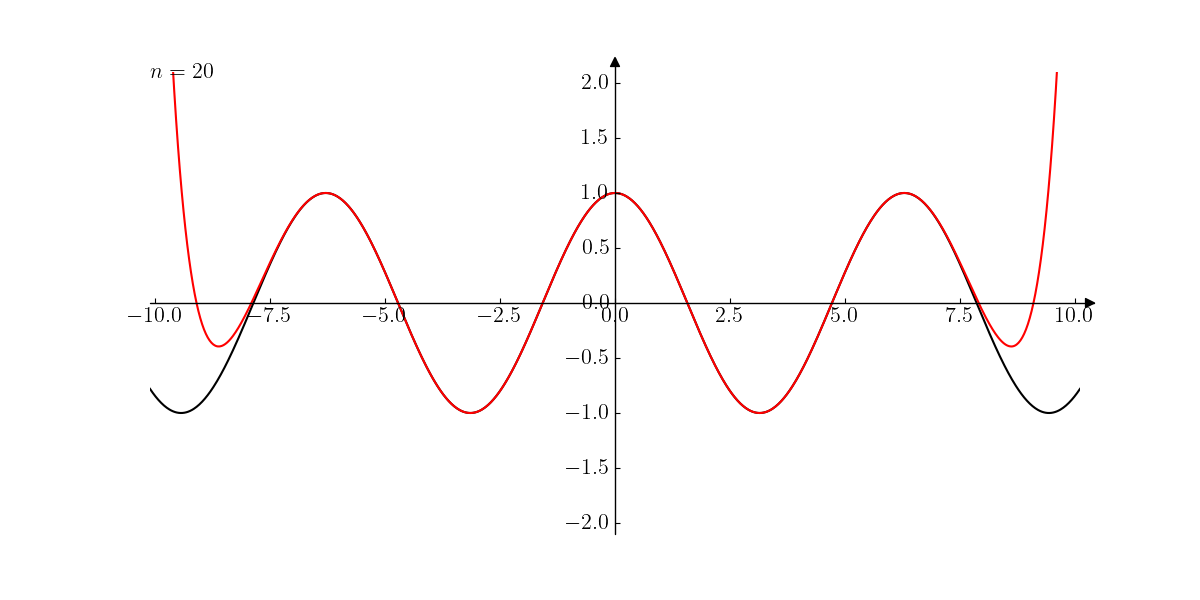
\includegraphics[scale=0.35]{./imagenes/TaylorCos_n20.png}
      \caption{$\cos(x)$ con su polinomio de Taylor de grado 20}
    \end{figure}
  \end{center}
\end{frame}

\begin{frame}
  \begin{egs}
    Encuentre la serie de Taylor de las siguientes funciones\\[0.5cm]
    \begin{itemize}[<+->]
      \item $e^x$\\[0.25cm]
      \item $\cos(x)$\\[0.25cm]
      \item $\sen(x)$\\[0.25cm]
      \item $\dfrac{1}{1+x^2}$\\[0.25cm]
      \item $\arctan(x)$\\[0.25cm]
    \end{itemize}
  \end{egs}
\end{frame}

\begin{frame}{Series de Taylor de funciones importantes}
  $$\begin{array}{|cccc|}
    \hline
    \text{función } & & \text{serie} & \text{intervalo convergencia}\\
    \hline
    & & & \\
    \dfrac{1}{1-x} & & \displaystyle\sum_{n=0}^\infty x^n & (-1,1)\\
    & & & \\
    e^x & & \displaystyle\sum_{n=0}^\infty \frac{x^n}{n!} & \Real\\
    & & & \\
    \sen(x) & & \displaystyle\sum_{n=0}^\infty (-1)^n\frac{x^{2n+1}}{(2n+1)!} & \Real\\
    & & & \\
    \cos(x) & & \displaystyle\sum_{n=0}^\infty (-1)^n\frac{x^{2n}}{(2n)!} & \Real\\
    & & & \\
    \hline
  \end{array}$$
\end{frame}

\begin{frame}{Series de Taylor de funciones importantes}
  $$\begin{array}{|cccc|}
    \hline
    \text{función } & & \text{serie} & \text{intervalo convergencia}\\
    \hline
    & & & \\
    \ln(1+x) & & \displaystyle\sum_{n=1}^\infty (-1)^{n-1}\frac{x^n}{n} & ]-1,1]\\
    & & & \\
    \arctan(x) & & \displaystyle\sum_{n=0}^\infty (-1)^n\frac{x^{2n+1}}{2n+1} & [-1,1]\\
    & & & \\
    \hline
  \end{array}$$
\end{frame}

%! subsección
\subsection{Ejercicios}
\begin{frame}
\subsectionpage
\end{frame}

% \begin{frame}
% \tableofcontents[currentsubsection]
% \end{frame}

\begin{frame}
  \begin{enumerate}
    \item Determine el radio y el intervalo de convergencia de las series
      % \begin{multicols}{2}
        \begin{enumerate}
          \item $\displaystyle\sum_{n=1}^\infty\dfrac{x^n}{n3^n}$
          \item $\displaystyle\sum_{n=1}^\infty n^n x^n$
          \item $\displaystyle\sum_{n=1}^\infty\dfrac{(-1)^n}{n}x^{2n}$
          \item $\displaystyle\sum_{n=1}^\infty\dfrac{(-1)^n}{n^2}(3x-1)^{n}$
        \end{enumerate}
      % \end{multicols}
  \end{enumerate}
\end{frame}


\begin{frame}
  \begin{enumerate}
    \setcounter{enumi}{1}
    \item Encuentre una representación en series de potencias para la función $\dfrac{2}{3-x}$ y determine su radio de convergencia.\\[0.5cm]
    \item Encuentre la representación en serie de Taylor de
    $$f(x)=\int e^{t^2}dt$$
    \item Las funciones $\cosh(x)$ y $\senh(x)$ se definen como
    $$\cosh(x)=\dfrac{e^x+e^{-x}}{2}\quad\text{y}\quad\senh(x)=\dfrac{e^x-e^{-x}}{2}$$
    Encuentre los polinomios de Taylor de grado $4$ y grado $n$ para $\cosh(x)$ centrados en $x=0$.
  \end{enumerate}
\end{frame}

% %! sección
% \section{Ejercicios de Repaso}
% \begin{frame}
% \sectionpage
% \end{frame}

% % \begin{frame}
% % \tableofcontents[currentsection]
% % \end{frame}

% %! subsección
% % \subsection{Ejercicios}
% % \begin{frame}
% % \subsectionpage
% % \end{frame}

% % \begin{frame}
% % \tableofcontents[currentsubsection]
% % \end{frame}

% \begin{frame}
% \end{frame}

\end{document}